\documentclass[12pt,a4paper]{report}
\usepackage[total={16.5cm,25.2cm}, top=2.5cm, left=2.5cm]{geometry}
\usepackage[czech]{babel}
\usepackage[T1]{fontenc}
\usepackage[utf8]{inputenc}
\usepackage{graphicx}
\usepackage{subcaption}
\usepackage{amsmath}
\usepackage{url}


\setlength\parindent{0.5cm} % šířka odsazení prvního řádku odstavce
\linespread{1.25} % řádkování 1.5 dle MS Word


%%% Údaje o práci
% Název práce v jazyce práce (přesně podle zadání)
\def\NazevPrace{Regresní neuronové sítě}
% Jméno autora
\def\AutorPrace{Lukáš Caha}
% Třída autora
\def\TridaAutora{8.M}
% Školní rok
\def\SkolniRok{2017/2018}
% Seminář ve kterém práce vznikla
\def\Seminar{Seminář z programování}
% Datum dokončení práce
\def\DatumDokonceni{\today}


%% Definice různých užitečných maker (viz popis uvnitř souboru)
%%% Tento soubor obsahuje definice různých užitečných maker a prostředí %%%
%%% Další makra připisujte sem, ať nepřekáží v ostatních souborech.     %%%

%%% Užitečné balíčky (jsou součástí běžných distribucí LaTeXu)
\usepackage{graphicx}       % vkládání obrázků
\usepackage{indentfirst}    % zavede odsazení 1. odstavce kapitoly
\usepackage[nottoc]{tocbibind} % zajistí přidání seznamu literatury,obrázků a tabulek do obsahu
\let\openright=\clearpage
\usepackage{hyperref}
\hypersetup{unicode}
\hypersetup{breaklinks=true}

%%% Drobné úpravy stylu

% Tato makra přesvědčují mírně ošklivým trikem LaTeX, aby hlavičky kapitol
% sázel příčetněji a nevynechával nad nimi spoustu místa. Směle ignorujte.
\makeatletter
\def\@makechapterhead#1{
  {\parindent \z@ \raggedright \normalfont
   \Huge\bfseries \thechapter. #1
   \par\nobreak
   \vskip 20\p@
}}
\def\@makeschapterhead#1{
  {\parindent \z@ \raggedright \normalfont
   \Huge\bfseries #1
   \par\nobreak
   \vskip 20\p@
}}
\makeatother

% Toto makro definuje kapitolu, která není očíslovaná, ale je uvedena v obsahu.
\def\chapwithtoc#1{
\chapter*{#1}
\addcontentsline{toc}{chapter}{#1}
}

% Trochu volnější nastavení dělení slov, než je default.
\lefthyphenmin=2
\righthyphenmin=2

% Zapne černé "slimáky" na koncích řádků, které přetekly, abychom si
% jich lépe všimli.
\overfullrule=1mm




\begin{document}

%% Titulní strana a různé povinné informační strany
%%% Titulní strana práce a další povinné informační strany

%%% Titulní strana práce

\pagestyle{empty}
\hypersetup{pageanchor=false}

\begin{center}

{\large\textbf{Gymnázium Christiana Dopplera, Zborovská 45, Praha 5}}

\vspace{70mm}

{\Large ROČNÍKOVÁ PRÁCE}
\\ \vspace{4mm}
{\Huge\bfseries\NazevPrace}

\vfill
\end{center}

\begin{tabular}{ll}
Vypracoval: & \AutorPrace \\
Třída: & \TridaAutora \\
Školní rok: & \SkolniRok \\
Seminář: & \Seminar \\
\end{tabular}
\newpage

%%% Strana s čestným prohlášením k diplomové práci
\openright
\hypersetup{pageanchor=true}
\pagestyle{plain}
\pagenumbering{gobble}
\vglue 0pt plus 1fill

\noindent
Prohlašuji, že jsem svou ročníkovou práci napsal samostatně a výhradně s~použitím citovaných pramenů. Souhlasím s~využíváním práce na Gymnáziu Christiana Dopplera pro studijní účely.
\vspace{10mm}

\noindent V Praze dne \DatumDokonceni
\hfill
\AutorPrace

\vspace{10mm}
\noindent \hfill . . . . . . . . . . . . . . . . . .

\vspace{20mm}
\newpage

\openright
\pagestyle{plain}
\pagenumbering{arabic}
\setcounter{page}{2}


%%% Strana s automaticky generovaným obsahem diplomové práce
\tableofcontents

\chapter{Úvod}
Ve světě se nachází mnoho dat v mnoha podobách a v dnešní době se dostáváme do bodu, kdy nestačíme všechny třídit a využívat na 100 \%.

Neuronové sítě jsou vrcholem lidské práce v oblasti informačních technologií. Mohl bych je přirovnat k lidskému mozku. A důvodem proč je zde zmiňuji je právě jejich všestranost. Sítí můžeme pouštět dva typy dat. Jedak lidmi vyhodnocené, a poté nevyhodnocené u nichž budu chtít výsledek. Neuronové sítě se podle prvního typu dat naučí jaká je souvislost mezi vstupem a výstupem a pak můžou přibližně určit výstupy dat druhého typu. Pokud byla v prvé řadě síť správně designovaná můžeme očekávat výsledky s poměrně velikou přesností a rychlostí zpracování, na jakou jsem zvyklí u počítačů.

Touto prací bych chtěl rozebrat neuronové sítě na úroveň pochopitelnou i pro středoškoláky, kteří by chtěli začít se strojovým učením, což je obor zahrnující moderní způsoby práce s umělou inteligencí.

\chapter{Základní pojmy} % NÁZVY KAPITOL NEJVYŠŠÍ ÚROVNĚ

\section{Neuron}
	\begin{figure}[h]
		\centering
		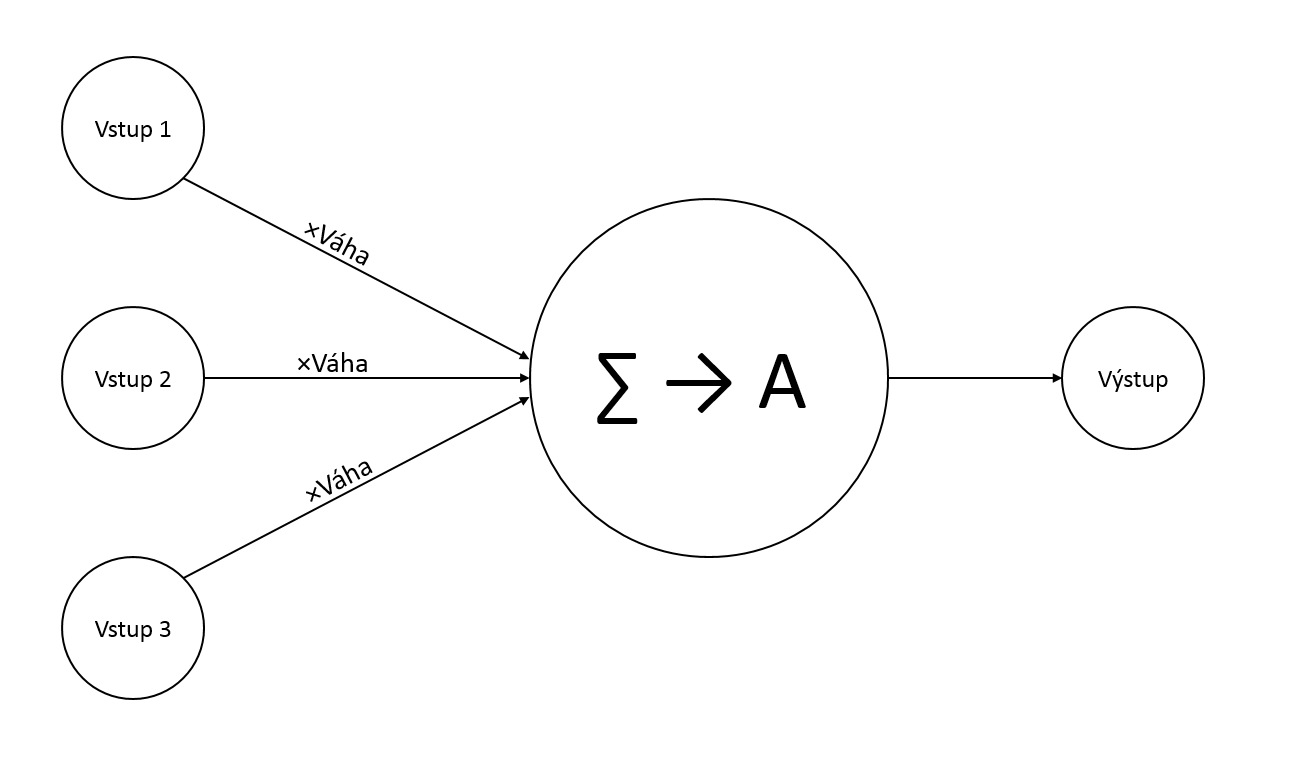
\includegraphics[width=10cm]{neuron}
		\caption{Diagram neuronu}
	\end{figure}
	\subsection{Jádro}
		\paragraph{Aktivace}
		je hodnota rozumně blízko nule $(a=0.73)$. Tahle hodnota určuje míru zapnutosti neuronu. Více aktivované neurony můžou mít větší vliv na neurony v sítí přímo následující. Aktivace neuronů jsou závislé na datech, takže není možné měnit jejich hodnoty přímo.
		\subsubsection{Aktivační funkce}
		Aktivační funkce upravuje příchozí signály, tak aby následně vytvořená hodnota zapadala řádů ostatních jednotek. Přijdou-li do neuronu 4 signály všechny s vyskou kladnou hodnotou, bude aktivace neuronu kladná a bude se blížit ostatním hodnotám vzniklým ze silných signálů.
		\paragraph{Signum}
		je nejzákladnější funkce, která může být pro tento úkol použita. Má všechny potřebné vlastnosti. Bohužel ztrácíme touto funkcí detail, který může být při tréningu sítě klíčový.
		\paragraph{Sigmoid}
		byla nejvíce používaná aktivační funkce na začátku vývoje neuronových sítí. Je také velice jednoduchá na pochopení. Dnes jí hlavně používáme pro určení pravděpodobností ve výstupní vrstvě, jelikož vrací pouze hodnoty v intervalu $\left<0,1\right>$.
		\paragraph{Rectifier}
		je dnes velice oblíbená funkce. V odborné literatuře se můžeme setkat s názvem RELU (REctified Linear Unit). Její výhoda je, že opravdu silný vstup se nezmění na obyčejnou hodnotu jakou je například u Sigmoidu 1. Při použítí této funkce se stává celý program jednoduše vypočitatelný jelikož bude použito jen porovnání, násobení a sčítání.
		\paragraph{Tanh}
		je jedna z málo funkcí, která vrací záporné hodnoty. Tento specifický znak se občas ukáže vhodný, ale pro nejzákladnější modely není důležité tuto funkci používat.
		\begin{figure}
			\centering
			\begin{subfigure}[h]{0.3\textwidth}
				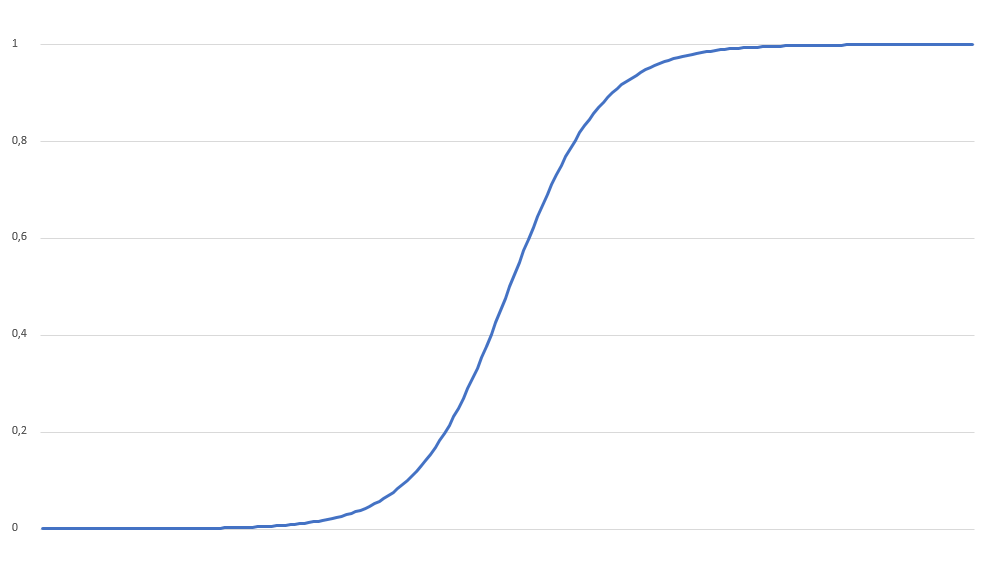
\includegraphics[width=\textwidth]{sigmoid}
				\caption{Sigmoid$=\frac{1}{1+e^{-x}}$}
				\label{fig:sigmoid}
			\end{subfigure}
			\begin{subfigure}[h]{0.3\textwidth}
				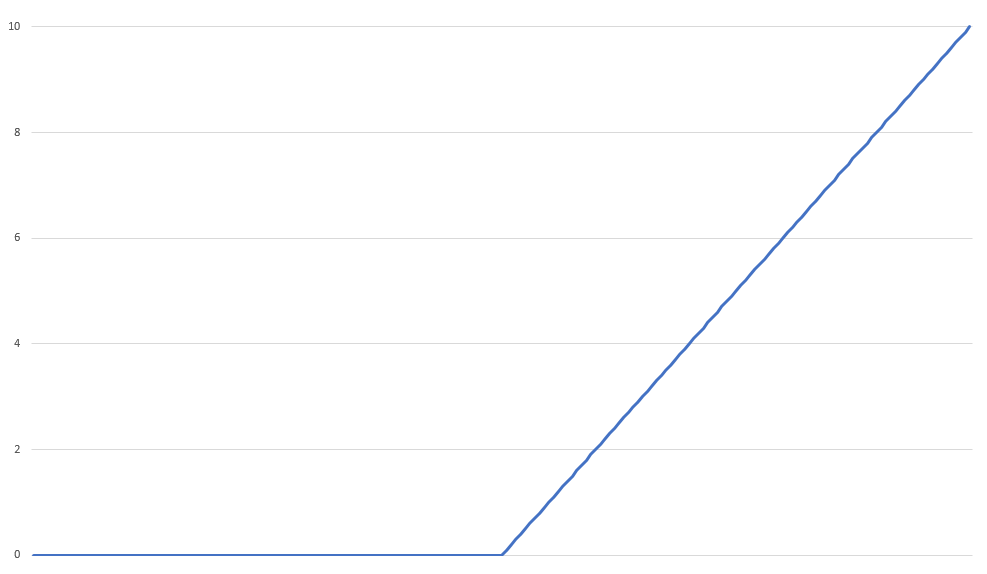
\includegraphics[width=\textwidth]{rectifier}
				\caption{Rectifier$=\max(0,x)$}
				\label{fig:rectifier}
			\end{subfigure}
			\begin{subfigure}[h]{0.3\textwidth}
				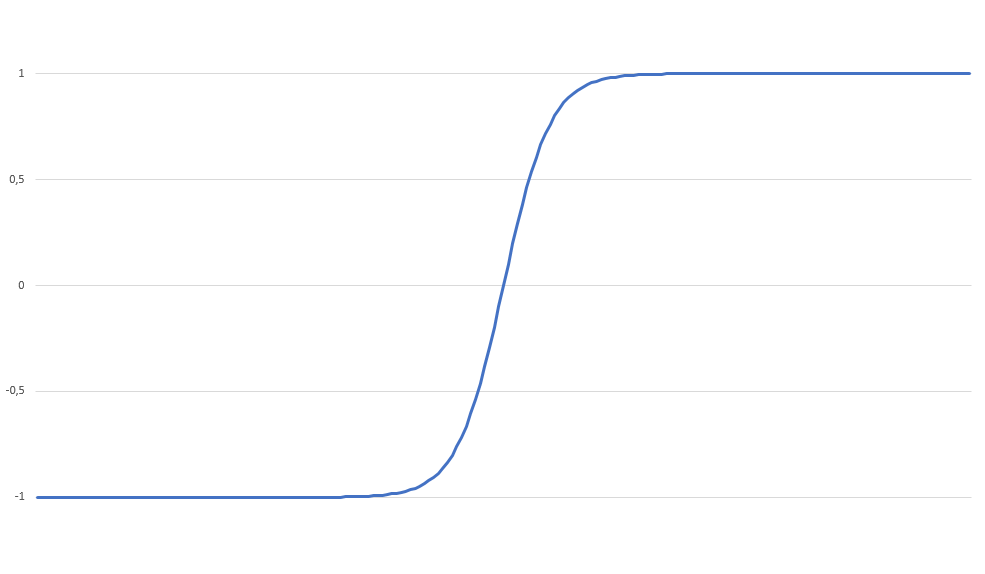
\includegraphics[width=\textwidth]{tanh}
				\caption{$\tanh(x)=\frac{e^{2x}-1}{e^{2x}+1}$}
				\label{fig:hyperbolic tangent}
			\end{subfigure}
			\caption{Aktivační funkce}\label{fig:activation functions}
		\end{figure}
	\subsection{Synapse}
		\paragraph{Synapse} je spojení mezi dvěma neurony. Toto spojení zajiťuje, že aktivace neuronu v síti je závislá na aktivacích předchozích neuronů.
		\paragraph{Váha}
		ovlivňuje spoje mezi neurony. Váhy spojení tvoří dohromady povahu sítě. Z libovolných vstupních dat můžu upravováním síly spojení (synapsí) vyvodit libovolné výstupní data. Mezi libovolnými dvoumi vrstvami je vždy plný počet synapsí a tedy i vah. Tento počet dostaneme vynásobením počtů neuronů v obou vrstvách.
\section{Síť}
	Síť se skládá s několik vrstev, které jsou navzájem propojené.
	\begin{figure}[h]
		\centering
		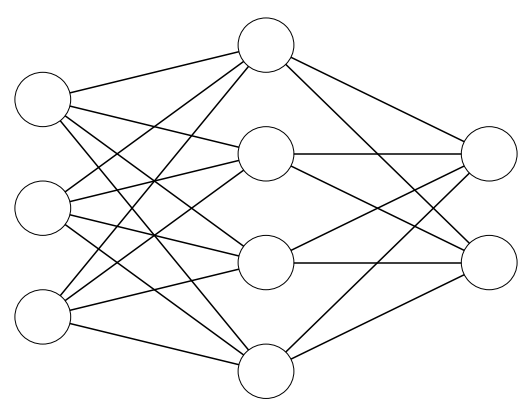
\includegraphics[width=10cm]{nn3-4-2}
		\caption{Diagram jednoduché sítě}
	\end{figure}
	\paragraph{Vrstva}
	je několik neuronů, které se navzájem neovlivňují, ale jsou ovlivněny stejnými neurony a zároveň ovlivňují stejé neurony.
	\paragraph{Bias}
	je míra vlivu nezávislého na datech. Tato externí síla se stará o vyrovnání sítí s menším počtem neuronů a tím uspoří výpočetní výkon. V překladu je bias šum, který rozostřuje data, aby se výsledná síť nepřizpůsobila až příliš moc trénovacím datům.
		
\section{Pohyb dat}
	\subsection{Vstup}
		\subsubsection{Typy vstupních dat}
			\paragraph{Trénovací data}
			jsou data u nichž používáme vstupy i výstupy pro vylepšování sítě. Pokud výsledná síť uvidí znovu tato data bude na nich mít mnohem lepší výsledky, jelikož je trénovaná speciálně na tyto data a až jako vedlejší produkt je tréning na data podobná.
			\paragraph{Testovací data}
			je soubor vstupů, u nichž je známý i výsledek. Ten ale nikdy není ukázán síti, slouží totiž pro porovnání výsledku sítě s pravidvým výsledkem. Takto získává uživatel statistiky o kvalitě sítě.
			\paragraph{Produkční data}
			jsou důvod proč síť vůbec programujeme. Tyto data dostává síť během běžného používání a počítá k nim výsledky. Není však možnost určit jak by tyto výsledky měli vyjít, a proto nám už zbývá pouze doufat, že síť funguje jak popisuje teorie.
		\paragraph{Scaling}
		je metoda upravení hodnot z našich vstupních dat, tak aby v síti tato data vystupovala pouze jako aktivace. Dobrým příkladem je vstupní hodnota věk. V našich datech se vyskytuje člověk s maximální věkem 100 a minimálním 0. Odpovídající hodnoty aktivace potom budou $100\rightarrow1.0$ a $0\rightarrow0.0$.
	\subsection{Výstup}
		\paragraph{Back-scaling}
		je forma získání dat zpět z neuronové sítě. Pokud zrovna trénujeme, není nutné data získávat a pak je porovnávat s očekávanými výsledky, lepší způsob je očekávané výsledky převést na jazyk, kterým komunikuje síť. Tímto samozdřejmě myslím použít scaling a převést výsledek na hodnotu mezi nulou a jedničkou.
	
\chapter{Vstup}
	\section{Design vstupní vrstvy}
		\subsection{Velikost vrstvy}
		Do vstupní vrstvy musíme dát dostatečné množství neuronů, aby mohli obsáhnout všechny důležité informace. Pokud budu například používat jako data obrázky o velikosti $28\times 28$px, tak vhodný počet vstupních neuronů je 784, takto neztratím žádná data a dokonce budou mít takhle všechny pixely rovnocený vliv. Pokud budu, ale používat jako data databázi s údaji o osobě, bude mi stačit neuronů zhruba stejný počet jako je sloupců v databázi.
	\section{Scaling}
	Jak již dobře víme, scaling je používán na získání hodnot mezi 0 a 1 ze vstupních dat. Našim vstupním číslům by síť totiž nemusela rozumět hned od začátku, jelikož se věk uvádí v řádu desítek, ale výplaty dosahují přibližně o 4 řády více. Vlivy těchto vstupních hodnot budou značně odlišné, což způsobí nechtěné nepřesnosti. Až později pochopíme jak funguje teoretické učení sítě zjistíme, že se tomuto kroku můžeme vyhnout, avšak z praktických zkušeností pak usoudíme, že scaling je docela užitečný krok.
	\section{Data}
	U začátku designování a programování sítě stojí vždy nějaká data. Každý trochu pokročilý programátor jistě dokáže vyjmenovat desítky případů, kdy mu znalost dat ulehčila práci. Tato znalost je u neuronových sítí naprosto zásadní. Když nevím co moje data znamenají nemůžu čekat, že to strojové učení odhadne za mě.
	
	Zároveň se musím postarat, abych použil data pravdivá, ve kterých se můžou opravdu existovat korelace, které můžu potvrdit letmou úvahou. Budu-li trénovat síť na míchání barev, musím použít reálné data o míchání barev. Kdybych si výsledné barvy vymýšlel náhodně můžu čekat, že odhady sítě budou také celkem náhodné. Když se později poohlédneme za cestou od začátku do vytrénované sítě uvidíme, že dvě stejné sítě můžou být vytrénovány na dvě různé činnosti. Celkově bych to shnul upraveným příslovím: "Síť nepadá daleko od dat."
		\subsection{Trénovací}
		Tento pojem již známe. Pojďme se tedy podívat na příklad míchaní barev. Na trénovacích datech obzvlášť záleží. Musíme z existujících údajů tedy vybrat co nejvíc náhodně vzorky, jejichž smíchání bylo ovlivněno co nejvíce faktory. Jednoduše pokud si vyberu na trénovaní pouze temné barvy, nemůžu potom očekávat, že síť správně smíchá dvě světlé barvy.
		\subsection{Testovací}
		Právě na těchto datech se uvidí, zda byly dosavadní kroky provedené úspěšně. Dosavadnímy kroky myslím celý postup, jelikož testovací data přichází skoro až na konci vývoje sítě. Jsou to právě tyto data, která nám oznámí jak dobře jsme odvedli práci trénování. Pokud se však nenachází podobné korelace mezi trénovacími a testovacími daty, bude náš test sítě neúspěšný a budeme se muset vrátit zpět ke trénování.
\chapter{Forward-propagation}
	Je to právě tento postup, který nám umožňuje pracovat s neuoronovými sítěmi. V průběhu vývoje se snažíme, aby tato fáze proběhla co nejlépe. Je to totiž výpočet toho co si síť myslí. Když tedy spustíme forward-propagation na nějakých datech dostaneme na výstup pořád pár divných čísel, podobných těm co vzniknou scalováním. To můžeme ale jednoduše změnit back-scalingem, což nám poskytne opravdu výstup, jaký by se dal čekat od živé bytosti se slušným uvažováním. Tento výstup bude zezačátku pravděpodobně většinou chybný, ale postupem času a trénováním se dostaneme do bodu, kdy výsledky opravdu odpovídají realitě.
	
	Nakonec když je síť ve fázi produkce, což znamená, že je využívaná a už se nemění, nejsou všechny synapse tolik důležité. Dosahují totiž hodnot blízkých nule, což působí, jako by vůbec neexistovaly.
	\section{Typy sítí}
	Při náhledu do lidského mozku asi nenajdeme takhle hezky uspořádané sítě z rovnocených neuronů. Stále však reprezentují dostatečně na to, aby to celé mohlo fungovat. Je dobré vědět, že existují i jiné typy sítí. Existují modifikace jenž umožňují pracovat s pamětí, vracejí již propočítaná data, nebo sami uspořádavají síť za běhu.
		\subsection{Feed-forward}
		Tento typ je asi nejjednoduší případ využití neuronových sítí. Veškerá data postupují organizovaně dále do sítě a na konci dosáhnou výsledných neuronů.
		
		Už víme, jak funguje neuron i aktivační funkce. Můžeme si tedy popsat tento zásadní algoritmus složený z toho co už známe.
		
		Vezmeme data vložené do vstupní vrstvy, která se na diagramech značí nalevo a postupujeme podle čar doprava. Postupně vezmeme každou synapsi, co se v diagramu vyskytuje mezi vrstvami jenž právě počítáme, a vynásobíme její váhu s aktivací levého neuronu a přičteme do pravého neuronu, kde je na začátku nula. Poté co vyhodnotíme všechny synapse aplikujeme na každý neuron pravé vrstvy aktivační funkci. Když dojdeme do konce, úspěšně jsme vyhodnotili jeden vstup.
		
		Při reprezentaci postupu pomocí programu můžeme využít násobení matice vrstvy s maticí vah a dostat tak výstupní vrstvu. Tímto způsobem můžeme zapsat zpracování libovolné vrstvy feed-forward modelu na jeden řádek.
		$$
		A_{vstup}
		\begin{bmatrix}
		1 & 2 & 3 & 4
		\end{bmatrix}
		\times
		W_{vstup}
		\begin{bmatrix}
		0  & 1 & -1 & 1  & 0  \\
		3  & 1 & 0  & 0  & 2  \\
		-1 & 2 & -3 & 0  & -1 \\
		1  & 2 & -1 & -2 & 0 
		\end{bmatrix}
		=
		A_{vrstva_1}
		\begin{bmatrix}
		7 & 5 & -14 & -7 & 1
		\end{bmatrix}
		$$
		
		Na tuto matici stačí uplatnit aktivační funkci a pokračovat dalším násobením.
		
		\subsection{Deep learning}
		Od slova deep (hluboké) jsou tyto sítě používány na zpracování komplikovanějších dat, jako je například rozpoznávání znaků. Uvnitř mají totiž více vrstev a každá funguje jako vstupní vrstva pro další. Takto si můžou jednotivé vrstvy předpracovat data a vrstva s výstupem už jen posbírá skoro hotové výsledky.
		\begin{figure}[h]
			\centering
			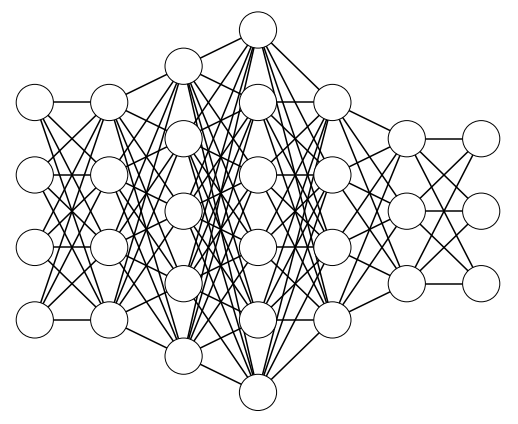
\includegraphics[width=15cm]{nn4-4-5-6-4-3-3}
			\caption{Více vrstev tvoří hloubku sítě}
		\end{figure}
\chapter{Back-propagation}
Použitím této metody můžeme síť opravdu něco naučit. Stručně řečeno si síť porovná výsledky s očekáváními a poté upraví váhy v síťi, tak aby nám další feed-forward fungoval trochu lépe.
	\section{Loss function}
	Celá síť je naprosto definovaná svým rozložením a vahami jednotlivých synapsí. Rozložení je fixní, takže pokud chceme ze sítě dostat maximum musíme upravovat váhy. Není však žádný jasný směr, kterým se vydat. Váh v síti je často od stovek k tisícům. Proto si zavedeme funkci loss neboli ztrátu. Tato funkce nám říká, jak moc je výsledek špatný. A najitím minimální hodnoty můžeme najít ideální stav sítě.
	\paragraph{Kvadratická ztrátová funkce}
	je nejčastěji používaná funkce. Její jednoduchost a lehká pochopitelnost jí staví nad všechny ostatní funkce, které můžou být pro určité případy lepší. $y$ je očekávaný výstup, $\hat{y}$ je vypočítaný výstup.
	$$L(y,\hat{y})=\frac{1}{2}(y-\hat{y})^2$$
	V případě, že máme více výstupních neuronů, je $L$ rovna sumě jednotlivých ztrát neuronů. Lineární multiplikátor $\frac{1}{2}$ je zde pouze pro zjednodušení pozdější derivace.
	
	\section{Prakticky}
	Pokud bych chtěl vysvětlit tento postup bez použití složité matematiky, můžu použít uvažování o vlivu jednotlivých chyb na výsledek sítě. Spočítám si pro každý neuron ve výstupní vrstvě o kolik a jakým směrem ho musím změnit, abych dosáhl správného výsledku. Pomocí synapsí vedoucích do předchozí vrstvy vypočítám, jak moc ovlivnili neurony v předchozí vrstvě tento výsledek.
	
	Neurony v předchozí vrstvě označím $a_1$ až $a_m$, neurony v této vrstvě $b_1$ až $b_n$. Váhu mezi neuronem $a_k$ z první vrstvy a neuronem $b_l$ z této vrstvy oznáčím $w_{k,l}$.
	
	Algoritmus v programu by mohl vypadat následnovně:
	\begin{enumerate}
		\item V každém z neuronů $a_1$ až $a_m$ si vytvořím proměnnou $d=0$, do které budu zapisovat, jak chtějí neurony $b$, aby vypadala aktivace (její relativní změna)
		\item Vezmu neuron $b_1$ a do proměnné $d_1$ neuronů $a_1$ až $a_m$ připíšu hodnotu váhy mezi neurony $d_1=d_1+w_{k,1}$
		\item Opakuji pro neurony $b_2$ až $b_n$
	\end{enumerate}
	Tímto jsem do každého neuronu v předposlední vrstvě získal předsavu výstupní vrstvy o ideálním stavu pro tento vstup. Postup zopakuju pro všechny ostatní vrstvy, s tím, že současná předchozí vrstva se stane výstupní vrstvou. Když dojdeme k počítání vytoužených aktivací mezi vstupní vrstvou a první počítací vrstvou nemůžeme už měnit nic jiného, než váhy. Proto nastavím váhy tak, aby z aktivovaných vstupních neuronů byly kladné váhy do neuronů co mají být aktivované a negativní váhy do neuronů co mají být vypnuté. Ze slabě aktivovaných vstupních neuronů nemusím měnit nic, protože nemají vliv na současnou situaci. Místo toho si je můžu ponechat pro jiné vstupní data, protože tam můžou mít vliv větší.
	
	Tímto postupem se můžu přiblížit k vytoužené síti, ale nevyužívám její plnou komplexitu. Proto můžu upravit i váhy v jiných vrstvách, než je mezi vstupní a první. Použiju úplně stejný postup. Pokud je neuron aktivovaný více nastavím váhu z něj do výstupů, co mají být aktivované trochu větší a do výstupů co mají být méně aktivované nastavím menší váhu.
	
	Během upravování všech vah používám významnou konstantu nazvanou "learning rate", která určuje, jak rychle se bude síť učit. Touto konstantou násobím všechny změny, jelikož rychlé změny v síti můžou způsobit zapomenutí informací, jenž se naučil dříve.

\chapter{Overfitting}
Po tom co síť vytrénujeme s velikou přesností nad $95\%$ na trénovacích datech, můžeme se radovat z velikého úspěchu. To ale není ještě výhra. Přesnost sítě se totiž musí hodnotit na datech testovacích. Během tréningu se totiž síť jako vedlejší produkt učí nazpaměť vstupy. Proto musíme v testu mít jiná data.

To znamená, že pokud máme vysokou úspěšnost na tréningu, ale nízkou na testu jsme obětí overfittingu. Do lidského uvažování to můžu přeložit, jako že program usoudil, že mu nedáváme dostatek dat na zjištění souvislostí a tak se naučil všechny vstupní data nazpaměť. Samozřejmě to znamená, že pokud programu nechám vyhodnotit i jednoduchou úlohu, tak nám nebude schopen odpovědět, pokud už takový příklad neviděl.

	\section{Řešení}
	Na předejití overfittingu existuje několik triků. Nejlepší by bylo použít od každého alespoň trochu.
	\begin{itemize}
		\item Přidáním vzorových dat
		\item Kontrolou, jestli jsou data relevantní
		\item Odstraněním vstupních hodnot, které nemají velký vliv
		\item Zastavením tréningu dřív, kdy test dosahuje dostatečně vysokých výsledků
	\end{itemize}
	

\chapter{Doporučení k programování}
	\section{Jazyk}
	Jako vývojový jazyk jsem si zvolil Python. Konkrétně používám verzi 3.6.3 na operačním systému Windows 7 64-bit. Tento jazyk jsem si zvolil především, protože je v oboru výrazně preferovaný. Tomu odpovídá i množství knihoven, které pro Python v oblasti strojového učení vzniklo. Běh Pythonu není nejrychlejší, ale při odhadu úspory času na běhu u jiných jazyků zase ztrácím čas na psaní velkého množství kódu.
		\subsection{Vývojové prostředí}
		Pro vývoj používám prostředí Spyder, které již podle názvu "Scientific PYthon Development EnviRonment" bylo navrženo čistě pro práci s Pythonem. Dva nejdůležitější nástroje poskytnuté prostředím jsou IPython console a Variable explorer. Instalaci jsem provedl skrz Pythnovou platformu pro data science jménem Anaconda.
		\paragraph{IPython console}
		umožňuje mít program zapnutý po celou dobu práce s modelem neuronové sítě. Ze začátku se zapne Python kernel, do kterého postupně nahráváme řádky kódu a ty se vyhodnocují. Styl jakým se nejčastějí píše kód z tohoto nástroje velmi benefituje. Jednotlivé části kódu na sebe totiž navazují, a proto je píšeme postupně. S náhledem do již vyhodnocené části kódu se nám následující program bude psát i opravovat rychleji. Tento nástroj opravdu oceníme, až budeme chtít upravit výpis dlouho trénované neuronové sítě, bez nutnosti pouštět celý program znovu.
		\paragraph{Variable explorer}
		nám dovolí dívat se živě na proměnné, které v programu existují. Největší uplatnění je asi na začátku, když se snažíme dostat data ze souboru do vstupní vrstvy a můžeme se dívat v jaké fázi se zrovna nachází.
		\subsection{Knihovny}
		Knihovny usnadňují práci s programem. Můžeme si je představit právě jako knihy z knihovny plné funkcí, které jsou většinou velmi jednoduché, ale i přes to vyžadují čas na vytvoření a organizaci zdrojových souborů. Navíc jsou dost často optimalizované na to co dělají.
			\paragraph{Pandas}
			čte vstupní soubory a nahrává data do lehce čitelných proměnných.
			\paragraph{NumPy}
			poskytuje značné množství jednoduchých matematických operací a funkcí, ze kterých je strojové učení složené.
			\paragraph{Scikit-learn}
			je podstatná knihovna pro práci s daty. Do tohoto oboru spadají i neuronové sítě. Využívám ji na rozdělení dat na testovací a trénovací, a také pro určení chyby a účinosti vytrénované sítě.
			\paragraph{Keras}
			je velmi pokročilá knihovna určená přímo pro neuronové sítě. Běží na základě knihoven Tensorflow od Googlu a Theano. Umožní nám zaměřit se přímo na stavění sítí a modelů, místo toho, abychom všechno psali od začátku můžeme začít pouze s teoretickými znalostmi.
			\paragraph{MatPlotLib}
			není knihovna, co by se značně podílela na funkčnosti. Poskytuje nám však značné možnosti ve vykreslování statistických údajů pomocí grafů.
	\section{Git}
		Pro zálohování a verzování používám Git. Konkrétně webovou službu GitHub \url{github.com/LukasCaha/GCHD\_prace}, kde se nachází veškerý kód asociovaný k této práci.
		
\chapter{Konvoluční předzpracování}
	Aplikováním následujícího postupu získáme vstupní hodnoty do neuronové sítě. Hlavní důvody, proč to děláme jsou rovnou dva. Prvním je přečtení souvislostí mezi jednotlivými pixely. Tato znalost je naprosto klíčová, protože jinak by se síť mohla zaměřit na výrazné, ale s obrázkem naprosto nesouvisející prvky (například šum v nočních snímcích). Druhým důvodem je zmenšení počtu informací, ale zachování informací rozhodujících pro správnou identifikaci obrázku. Tento postup nám tedy zrychlí zpracování bez ztráty kvality.
	\section{Konvoluce}
		\paragraph{Konvoluce}
		je zpracování dvou signálů na základě jejich průniku. V matematice se s konvolucí setkáváme jako s operátorem pro dvě funkce. První funkci nazýváme obraz a druhou filtr. Při filtru na obrázku můžeme dosáhnout například zvýraznění hran. Tento filtr tedy hledá hrany.
		\paragraph{Využití}
		je v mém případě hledání rysů na obrázku. Na hodně exaktní předloze můžu najít pomocí specifických filterů například přechod mezi nebem a mořem. Poté můžu do této oblasti přidat červený odstín pro zdůraznění západu slunce.
		
		Ve spojení s neuronovými sítěmi můžu automaticky určovat obsah obrázků. Na vstupní obrázek uplatním několik předem vytrénovaných filterů. Každý z nich zvýrazní oblasti obrázku, kde nalezl shodu. Při designu konvoluční vrstvy nastavujeme několik parametrů.
		
		\paragraph{Velikost filteru}
		záleží na uvážení, jestli spolu jednotlivé části obrázku souvisí hodně nebo málo.
		\paragraph{Počet filterů}
		určuje kolik filterů bude využito pro hledání znaků v obrázcích. Čím více jich bude, tím déle program poběží, ale budeme mít více rysů na kombinování.
	\section{Sdružování}
	 	\paragraph{Sdružování}
	 	neboli pooling je způsob vyzdvižení důležitých rysů a zanedbání informací nedůležitých. Také mírně zvýší entropii, čímž umožní dvoum mírně různým obrázkům, aby po předzpracování vypadali stejně. Tímto algoritmem také dosáhneme největší úspory času, jelikož sdružovací hlavice dělá z $n^2$ ($n$ je malé přizozené číslo viz. obrázek) informací informaci jednu.

		Stejně jako u všech algoritmů, které zde používám je mnoho možností jak je nastavit a získat tím různé výsledky různě rychle.
		\paragraph{Velikost poolu}
		je nastavena tak, aby jsme neztratili příliš mnoho informací, ale aby program běžel dostatečně rychle. Obvykle je vhodná velikost $2\times2$. Můžeme samozřejmě použít mřížku $3\times3$. Obecně se ale doporučuje mít shodné rozměry.
	\section{Vložení do sítě}
		Nakonec vezmu všechny sdružené obrázky a poskládám je do jednorozměrného pole. Tohle pole je vstupní vrstva neuronové sítě, kterou již známe. Po dokončení trénování stačí vložit obrázek na začátek konvoluce a stejným postupem nám výjde odhad.
		
\chapter{Závěr}
Během psaní této práce jsem se naučil naprosté základy neuronových sítí a jejich fungování. Pro učení bych ze zkušeností doporučil četné video návody, které lze najít na internetu zcela zdarma. V rámci procvičování jsem vytvořil tři modely neuronových sítí s postupně se zvyšující složitostí.

První program se učil souvislosti, které vytváří logické brány mezi vsupem a výstupem. Přesnost byla okolo $70\%$, což bylo způsobeno nedostatečnou složitostí problému a omezeností vstupních hodnot. \url{github.com/LukasCaha/GCHD_prace/blob/master/src/net_logicgates.py}

Druhý pokus mířil trochu výš, kdy program určoval, zda jsou buňky v poli zaškrtnuté vertikálně symetricky. Vzhledem k jednoduchosti problému bylo jednoduché získat velký počet trénovacích a testovacích dat. To zapříčínilo úžasnou úspěšnost nad $99\%$ na testovacích datech. \url{github.com/LukasCaha/ANN_symetry}

Poslední počin mířil na počítačovou vizi (computer vizion), kde je účelem rozpoznat, zda je na obrázku pes, nebo kočka. Tento problém mi zabral nejvíce času, jelikož jsem se potýkal s dlouhou výpočetní dobou programu. Po asi deseti hodinách se mi tréningem podařilo získat testovací úspěšnost $80\%$, což považuji za veliký úspěch, vzhledem k tomu jak byl problém komplexní. \url{github.com/LukasCaha/GCHD_prace/blob/master/src/cnn.py}



%%% Seznam použité literatury
\begin{thebibliography}{99}

\bibitem{birge}
Birge J. R., Wets R. J.-B. (1987): Computing bounds for stochastic programing problems by means of a generalized moment problem. \textit{Mathematics of Operations Research} \textbf{12}, 149-162.
\end{thebibliography}

%%% Prostor pro přílohy práce
\chapwithtoc{Přílohy}

\openright
\end{document}
